% Neural network diagram
% Made with Xematics. Positions are in px (1 px = 0.75 pt), as in the SVG export.
\documentclass[tikz, border=4pt]{standalone}
\definecolor{xm1}{HTML}{FFFFFF}
\definecolor{xm2}{HTML}{E0F3EC}
\definecolor{xm3}{HTML}{00845F}
\definecolor{xm4}{HTML}{F7EAF2}
\definecolor{xm5}{HTML}{A8558A}
\definecolor{xm6}{HTML}{6B7280}
\definecolor{xm7}{HTML}{C9CCD0}
\definecolor{xm8}{HTML}{8F969E}
\definecolor{xm9}{HTML}{B7BBC1}
\definecolor{xm10}{HTML}{737A85}
\definecolor{xm11}{HTML}{A5AAB1}
\definecolor{xm12}{HTML}{C2C5CA}
\definecolor{xm13}{HTML}{858B95}
\definecolor{xm14}{HTML}{ACB1B7}
\definecolor{xm15}{HTML}{B8C0CC}
\definecolor{xm16}{HTML}{F1F2F4}
\definecolor{xm17}{HTML}{4B5563}
\definecolor{xm18}{HTML}{D4E8F5}
\definecolor{xm19}{HTML}{0072B2}
\definecolor{xm20}{HTML}{FBE8C4}
\definecolor{xm21}{HTML}{B97800}
\definecolor{xm22}{HTML}{D55E00}
\definecolor{xm23}{HTML}{1F2937}
\begin{document}
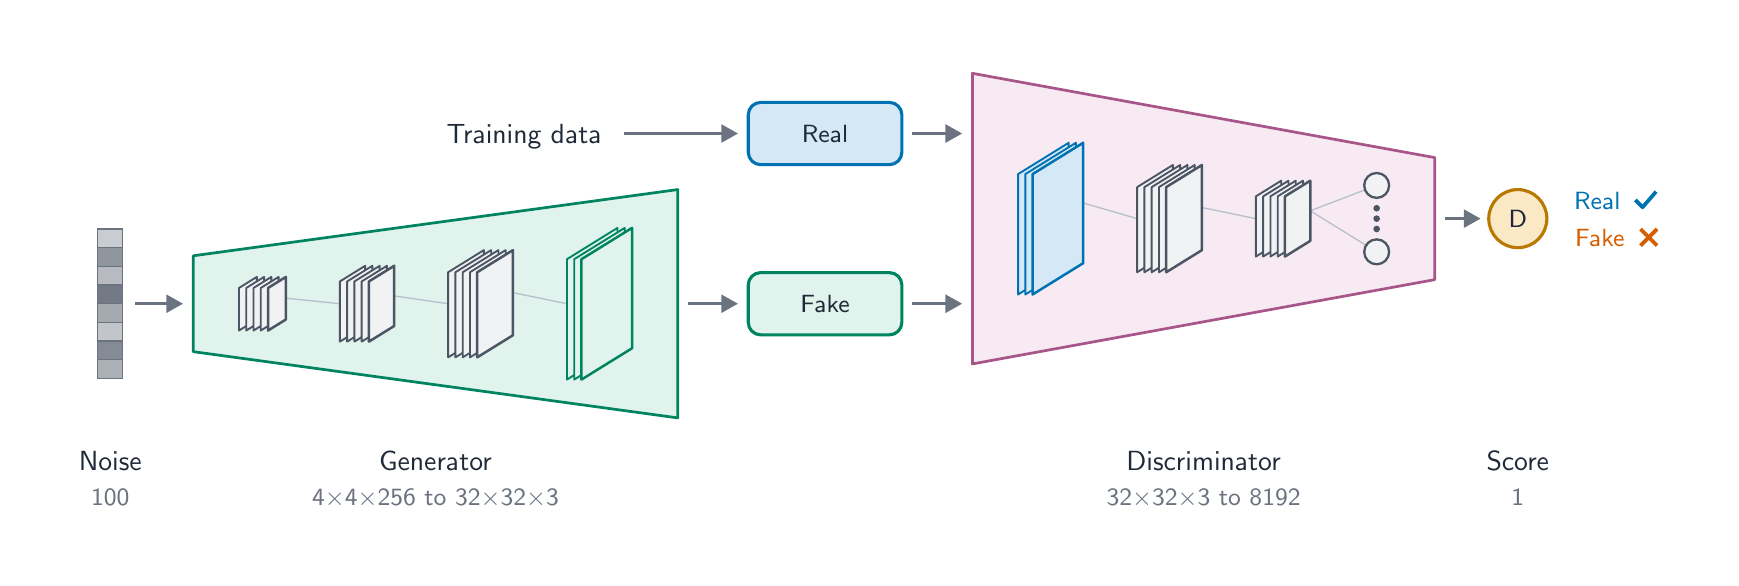
\begin{tikzpicture}[x=0.75pt, y=-0.75pt]
  \tikzset{
    xm funnel 18a79of/.style={fill=xm2, draw=xm3, line width=0.98pt, line join=round},
    xm funnel 1dcnepv/.style={fill=xm4, draw=xm5, line width=0.98pt, line join=round},
    xm arrow 1l69f7x/.style={draw=xm6, line width=1.05pt},
    xm arrow 19pejvw/.style={fill=xm6, line join=round},
    xm box 13pbqni/.style={fill=xm7, draw=xm6, line width=0.45pt},
    xm box 13w2a8d/.style={fill=xm8, draw=xm6, line width=0.45pt},
    xm box 142stt8/.style={fill=xm9, draw=xm6, line width=0.45pt},
    xm box 1unt8g8/.style={fill=xm10, draw=xm6, line width=0.45pt},
    xm box 1uujs13/.style={fill=xm11, draw=xm6, line width=0.45pt},
    xm box 1v1ably/.style={fill=xm12, draw=xm6, line width=0.45pt},
    xm box 1v80v6t/.style={fill=xm13, draw=xm6, line width=0.45pt},
    xm box 1verero/.style={fill=xm14, draw=xm6, line width=0.45pt},
    xm edge 170dxcz/.style={draw=xm15, line width=0.48pt},
    xm sheet 1fhs3ho/.style={fill=xm16, draw=xm17, line width=0.68pt, line join=round},
    xm sheet 1h1bm7r/.style={fill=xm16, draw=xm17, line width=0.9pt, line join=round},
    xm sheet xspbgc/.style={fill=xm2, draw=xm3, line width=0.68pt, line join=round},
    xm sheet fsyzdz/.style={fill=xm2, draw=xm3, line width=0.9pt, line join=round},
    xm box 442wj7/.style={fill=xm18, draw=xm19, line width=1.13pt, rounded corners=4.5pt},
    xm box 4erm6b/.style={fill=xm2, draw=xm3, line width=1.13pt, rounded corners=4.5pt},
    xm sheet nfv2b0/.style={fill=xm18, draw=xm19, line width=0.68pt, line join=round},
    xm sheet 14ob247/.style={fill=xm18, draw=xm19, line width=0.9pt, line join=round},
    xm node hvhhxc/.style={fill=xm16, draw=xm17, line width=0.83pt},
    xm circle 1g24ir9/.style={fill=xm17},
    xm node 1tdv5pi/.style={fill=xm20, draw=xm21, line width=1.13pt},
    xm mark moeldj/.style={draw=xm19, line width=1.35pt, line join=round},
    xm mark bi72rz/.style={draw=xm22, line width=1.35pt, line join=round},
    xm text xm23/.style={text=xm23, inner sep=0},
    xm text xm19/.style={text=xm19, inner sep=0},
    xm text xm22/.style={text=xm22, inner sep=0},
    xm text xm6/.style={text=xm6, inner sep=0},
  }
  \fill[xm1] (0,0) rectangle (811.05,255.25);
  % Diagram
  \path[xm funnel 18a79of] (79.8,109.9) -- (313.18,78) -- (313.18,188) -- (79.8,156.1) -- cycle;
  \path[xm funnel 1dcnepv] (455.18,22) -- (677.94,62.6) -- (677.94,121.4) -- (455.18,162) -- cycle;
  \path[xm arrow 1l69f7x] (51.8,133) -- (67.8,133);
  \path[xm arrow 19pejvw] (74.8,133) -- (66.8,137.5) -- (66.8,128.5) -- cycle;
  \path[xm arrow 1l69f7x] (318.18,133) -- (335.18,133);
  \path[xm arrow 19pejvw] (342.18,133) -- (334.18,137.5) -- (334.18,128.5) -- cycle;
  \path[xm arrow 1l69f7x] (426.18,133) -- (443.18,133);
  \path[xm arrow 19pejvw] (450.18,133) -- (442.18,137.5) -- (442.18,128.5) -- cycle;
  \path[xm arrow 1l69f7x] (426.18,51) -- (443.18,51);
  \path[xm arrow 19pejvw] (450.18,51) -- (442.18,55.5) -- (442.18,46.5) -- cycle;
  \path[xm arrow 1l69f7x] (287.18,51) -- (335.18,51);
  \path[xm arrow 19pejvw] (342.18,51) -- (334.18,55.5) -- (334.18,46.5) -- cycle;
  \path[xm arrow 1l69f7x] (682.94,92) -- (692.94,92);
  \path[xm arrow 19pejvw] (699.94,92) -- (691.94,96.5) -- (691.94,87.5) -- cycle;
  \path[xm box 13pbqni] (33.8,97) rectangle ++(12,9);
  \path[xm box 13w2a8d] (33.8,106) rectangle ++(12,9);
  \path[xm box 142stt8] (33.8,115) rectangle ++(12,9);
  \path[xm box 1unt8g8] (33.8,124) rectangle ++(12,9);
  \path[xm box 1uujs13] (33.8,133) rectangle ++(12,9);
  \path[xm box 1v1ably] (33.8,142) rectangle ++(12,9);
  \path[xm box 1v80v6t] (33.8,151) rectangle ++(12,9);
  \path[xm box 1verero] (33.8,160) rectangle ++(12,9);
  \path[xm edge 170dxcz] (124.41,130.33) -- (150.41,133);
  \path[xm edge 170dxcz] (176.59,129.23) -- (202.59,133);
  \path[xm edge 170dxcz] (233.82,127.67) -- (259.82,133);
  \path[xm sheet 1fhs3ho] (101.8,125.41) -- (110.41,120.08) -- (110.41,140.59) -- (101.8,145.92) -- cycle;
  \path[xm sheet 1fhs3ho] (105.3,125.41) -- (113.91,120.08) -- (113.91,140.59) -- (105.3,145.92) -- cycle;
  \path[xm sheet 1fhs3ho] (108.8,125.41) -- (117.41,120.08) -- (117.41,140.59) -- (108.8,145.92) -- cycle;
  \path[xm sheet 1fhs3ho] (112.3,125.41) -- (120.91,120.08) -- (120.91,140.59) -- (112.3,145.92) -- cycle;
  \path[xm sheet 1h1bm7r] (115.8,125.41) -- (124.41,120.08) -- (124.41,140.59) -- (115.8,145.92) -- cycle;
  \path[xm sheet 1fhs3ho] (150.41,122.27) -- (162.59,114.73) -- (162.59,143.73) -- (150.41,151.27) -- cycle;
  \path[xm sheet 1fhs3ho] (153.91,122.27) -- (166.09,114.73) -- (166.09,143.73) -- (153.91,151.27) -- cycle;
  \path[xm sheet 1fhs3ho] (157.41,122.27) -- (169.59,114.73) -- (169.59,143.73) -- (157.41,151.27) -- cycle;
  \path[xm sheet 1fhs3ho] (160.91,122.27) -- (173.09,114.73) -- (173.09,143.73) -- (160.91,151.27) -- cycle;
  \path[xm sheet 1h1bm7r] (164.41,122.27) -- (176.59,114.73) -- (176.59,143.73) -- (164.41,151.27) -- cycle;
  \path[xm sheet 1fhs3ho] (202.59,117.83) -- (219.82,107.16) -- (219.82,148.17) -- (202.59,158.84) -- cycle;
  \path[xm sheet 1fhs3ho] (206.09,117.83) -- (223.32,107.16) -- (223.32,148.17) -- (206.09,158.84) -- cycle;
  \path[xm sheet 1fhs3ho] (209.59,117.83) -- (226.82,107.16) -- (226.82,148.17) -- (209.59,158.84) -- cycle;
  \path[xm sheet 1fhs3ho] (213.09,117.83) -- (230.32,107.16) -- (230.32,148.17) -- (213.09,158.84) -- cycle;
  \path[xm sheet 1h1bm7r] (216.59,117.83) -- (233.82,107.16) -- (233.82,148.17) -- (216.59,158.84) -- cycle;
  \path[xm sheet xspbgc] (259.82,111.54) -- (284.18,96.46) -- (284.18,154.46) -- (259.82,169.54) -- cycle;
  \path[xm sheet xspbgc] (263.32,111.54) -- (287.68,96.46) -- (287.68,154.46) -- (263.32,169.54) -- cycle;
  \path[xm sheet fsyzdz] (266.82,111.54) -- (291.18,96.46) -- (291.18,154.46) -- (266.82,169.54) -- cycle;
  \path[xm box 442wj7] (347.18,36) rectangle ++(74,30);
  \path[xm box 4erm6b] (347.18,118) rectangle ++(74,30);
  \path[xm edge 170dxcz] (508.54,84.46) -- (534.54,92);
  \path[xm edge 170dxcz] (565.76,86.67) -- (591.76,92);
  \path[xm edge 170dxcz] (617.94,88.23) -- (644.34,78.14);
  \path[xm edge 170dxcz] (617.94,88.23) -- (644.84,104.85);
  \path[xm sheet nfv2b0] (477.18,70.54) -- (501.54,55.46) -- (501.54,113.46) -- (477.18,128.54) -- cycle;
  \path[xm sheet nfv2b0] (480.68,70.54) -- (505.04,55.46) -- (505.04,113.46) -- (480.68,128.54) -- cycle;
  \path[xm sheet 14ob247] (484.18,70.54) -- (508.54,55.46) -- (508.54,113.46) -- (484.18,128.54) -- cycle;
  \path[xm sheet 1fhs3ho] (534.54,76.83) -- (551.76,66.16) -- (551.76,107.17) -- (534.54,117.84) -- cycle;
  \path[xm sheet 1fhs3ho] (538.04,76.83) -- (555.26,66.16) -- (555.26,107.17) -- (538.04,117.84) -- cycle;
  \path[xm sheet 1fhs3ho] (541.54,76.83) -- (558.76,66.16) -- (558.76,107.17) -- (541.54,117.84) -- cycle;
  \path[xm sheet 1fhs3ho] (545.04,76.83) -- (562.26,66.16) -- (562.26,107.17) -- (545.04,117.84) -- cycle;
  \path[xm sheet 1h1bm7r] (548.54,76.83) -- (565.76,66.16) -- (565.76,107.17) -- (548.54,117.84) -- cycle;
  \path[xm sheet 1fhs3ho] (591.76,81.27) -- (603.94,73.73) -- (603.94,102.73) -- (591.76,110.27) -- cycle;
  \path[xm sheet 1fhs3ho] (595.26,81.27) -- (607.44,73.73) -- (607.44,102.73) -- (595.26,110.27) -- cycle;
  \path[xm sheet 1fhs3ho] (598.76,81.27) -- (610.94,73.73) -- (610.94,102.73) -- (598.76,110.27) -- cycle;
  \path[xm sheet 1fhs3ho] (602.26,81.27) -- (614.44,73.73) -- (614.44,102.73) -- (602.26,110.27) -- cycle;
  \path[xm sheet 1h1bm7r] (605.76,81.27) -- (617.94,73.73) -- (617.94,102.73) -- (605.76,110.27) -- cycle;
  \path[xm node hvhhxc] (649.94,76) circle[radius=6];
  \path[xm circle 1g24ir9] (649.94,87) circle[radius=1.6];
  \path[xm circle 1g24ir9] (649.94,92) circle[radius=1.6];
  \path[xm circle 1g24ir9] (649.94,97) circle[radius=1.6];
  \path[xm node hvhhxc] (649.94,108) circle[radius=6];
  \path[xm node 1tdv5pi] (717.94,92) circle[radius=14];
  \path[xm mark moeldj] (774.56,83) -- (778.06,86.5) -- (784.56,79);
  \path[xm mark bi72rz] (777.05,97) -- (785.05,105) (785.05,97) -- (777.05,105);
  \node[xm text xm23, font=\sffamily\fontsize{9}{10.8}\selectfont, anchor=base] at (384.18,55.37) {Real};
  \node[xm text xm23, font=\sffamily\fontsize{9}{10.8}\selectfont, anchor=base] at (384.18,137.37) {Fake};
  \node[xm text xm23, font=\sffamily\fontsize{9.75}{11.7}\selectfont, anchor=base] at (239.17,55.73) {Training data};
  \node[xm text xm23, font=\sffamily\fontsize{9}{10.8}\selectfont, anchor=base] at (717.94,96.37) {D};
  \node[xm text xm19, font=\sffamily\fontsize{9}{10.8}\selectfont, anchor=base] at (756.25,87.37) {Real};
  \node[xm text xm22, font=\sffamily\fontsize{9}{10.8}\selectfont, anchor=base] at (757.5,105.37) {Fake};
  \node[xm text xm23, font=\sffamily\fontsize{9.75}{11.7}\selectfont, anchor=base] at (39.8,213.59) {Noise};
  \node[xm text xm6, font=\sffamily\fontsize{9}{10.8}\selectfont, anchor=base] at (39.8,230.35) {100};
  \node[xm text xm23, font=\sffamily\fontsize{9.75}{11.7}\selectfont, anchor=base] at (196.49,213.59) {Generator};
  \node[xm text xm6, font=\sffamily\fontsize{9}{10.8}\selectfont, anchor=base] at (196.49,230.35) {4\ensuremath{\times}4\ensuremath{\times}256 to 32\ensuremath{\times}32\ensuremath{\times}3};
  \node[xm text xm23, font=\sffamily\fontsize{9.75}{11.7}\selectfont, anchor=base] at (566.56,213.59) {Discriminator};
  \node[xm text xm6, font=\sffamily\fontsize{9}{10.8}\selectfont, anchor=base] at (566.56,230.35) {32\ensuremath{\times}32\ensuremath{\times}3 to 8192};
  \node[xm text xm23, font=\sffamily\fontsize{9.75}{11.7}\selectfont, anchor=base] at (717.94,213.59) {Score};
  \node[xm text xm6, font=\sffamily\fontsize{9}{10.8}\selectfont, anchor=base] at (717.94,230.35) {1};
\end{tikzpicture}
\end{document}
